

%************************************************
\chapter{Machine Learning Theory}\label{ch:mlt}

%************************************************
\begin{quotation}
	\small \textit{ \flushright Mathematics operates inside the thin layer \\
	between the trivial and the intractable.\\
	\flushright --- Andrey Kolmogorov\\
	\vspace{1cm} }
\end{quotation}

In which we present the theoretical framework of Machine Learning, the PAC model, theoretical guarantees for generalisation, and expose criticism due to its lack of explanation on Deep Learning phenomena\footnote{This chapter is influenced by the online lecture~\citeauthor{shawe-taylor:2018}, the online lecture series~\citeauthor{mello:2018online} and the book~\citeauthor{mello:2018}. }.


\section{Motivation} As already discussed, learning is the process of inferring general rules to perform a specific task by observing limited examples. The learning algorithm must perform well in the sample already seen and, more importantly, in previously unseen examples.

How can we prove that an algorithm learned? We may know its performance in the given sample, but does it translate to any sample? Can we guarantee bounds to the error in an unknown distribution of examples even if we have just a limited sample of it? Can we bound the number of samples needed (sample complexity) to ensure accuracy on unseen examples? How does the sample complexity grow?
\begin{figure}[hbt!]
	\centering
	
\includegraphics[width=.6
	\textwidth]{vc2}
	\caption{Chervonenkis (Left) and Vapnik (Right).}\label{fig:VC}
\end{figure}
These are the kind of questions that motivated the development of Machine Learning Theory (MLT). This research field started in Russia by the name of Statistical Learning Theory (SLT), during the late \(1960_s\), with the work of Vapnik and Chervonenkis (see \cref{fig:VC}). In 1984, Leslie Valiant proposed the Probably Approximately Correct (PAC) framework to bring ideas from the Computational Complexity Theory to learning problems, giving birth to the field of Computational Learning Theory (CoLT). Up to the \(1990_s\), STL and CoLT were very active fields.
We will also limit our overview of MLT to the context of supervised binary classification problems. This limitation is not a deficiency of the theory but a mere choice of scope for this document.


\section {The Learning Problem}
The goal of learning is to understand the world from experience, coming up with a theory, a tested hypothesis.

\begin{figure}[ht]
	\centering
	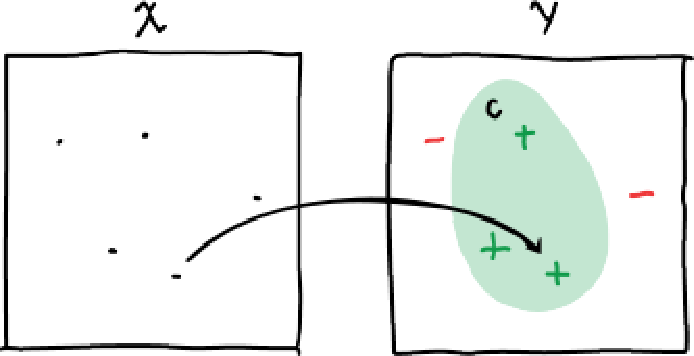
\includegraphics[width=0.45
	\textwidth]{concept}
	\caption{A \emph{concept} \(c\) is an idealised mapping from the input space \(\XX\) to output space \(\YY\). Each point on the left is an instance \(\rx_i\). Note that given that \(\YY\) is binary, \(c \subset \XX\).}
\end{figure}

The learning task is the \emph{concept} \(c\) we want to learn. The concept is the idealised function that maps an instance of the problem \(\rx_i\) from the input space \(\XX\) (also known as problem space) to a solution \(\ry_i\) of the output space \(\YY\) (also known as label space). In the PAC framework, the convention is that labels are binary, \(\YY = \{-, +\}\), therefore, \(c \subset \XX\). A concept class \(\CC\) is a set of concepts \(c\), thus, a set of sets of \(\XX\).

We imagine there is a certain distribution \(\DD = \PXY \) in nature, from which \(P(\rvX)\), the distribution of examples, and \(P(\rvY|\rvX)\), the learning task, derive. Even knowing nothing about \(\DD\), we want to discover \(P(\rvY|\rvX)\), given a sample of \((x, y) \sim \PXY\).

\subsection{The learning problem setting}

Supervised learning has three main components (see \cref{fig:problem_setting}):
\begin{figure}
	[ht] \centering
	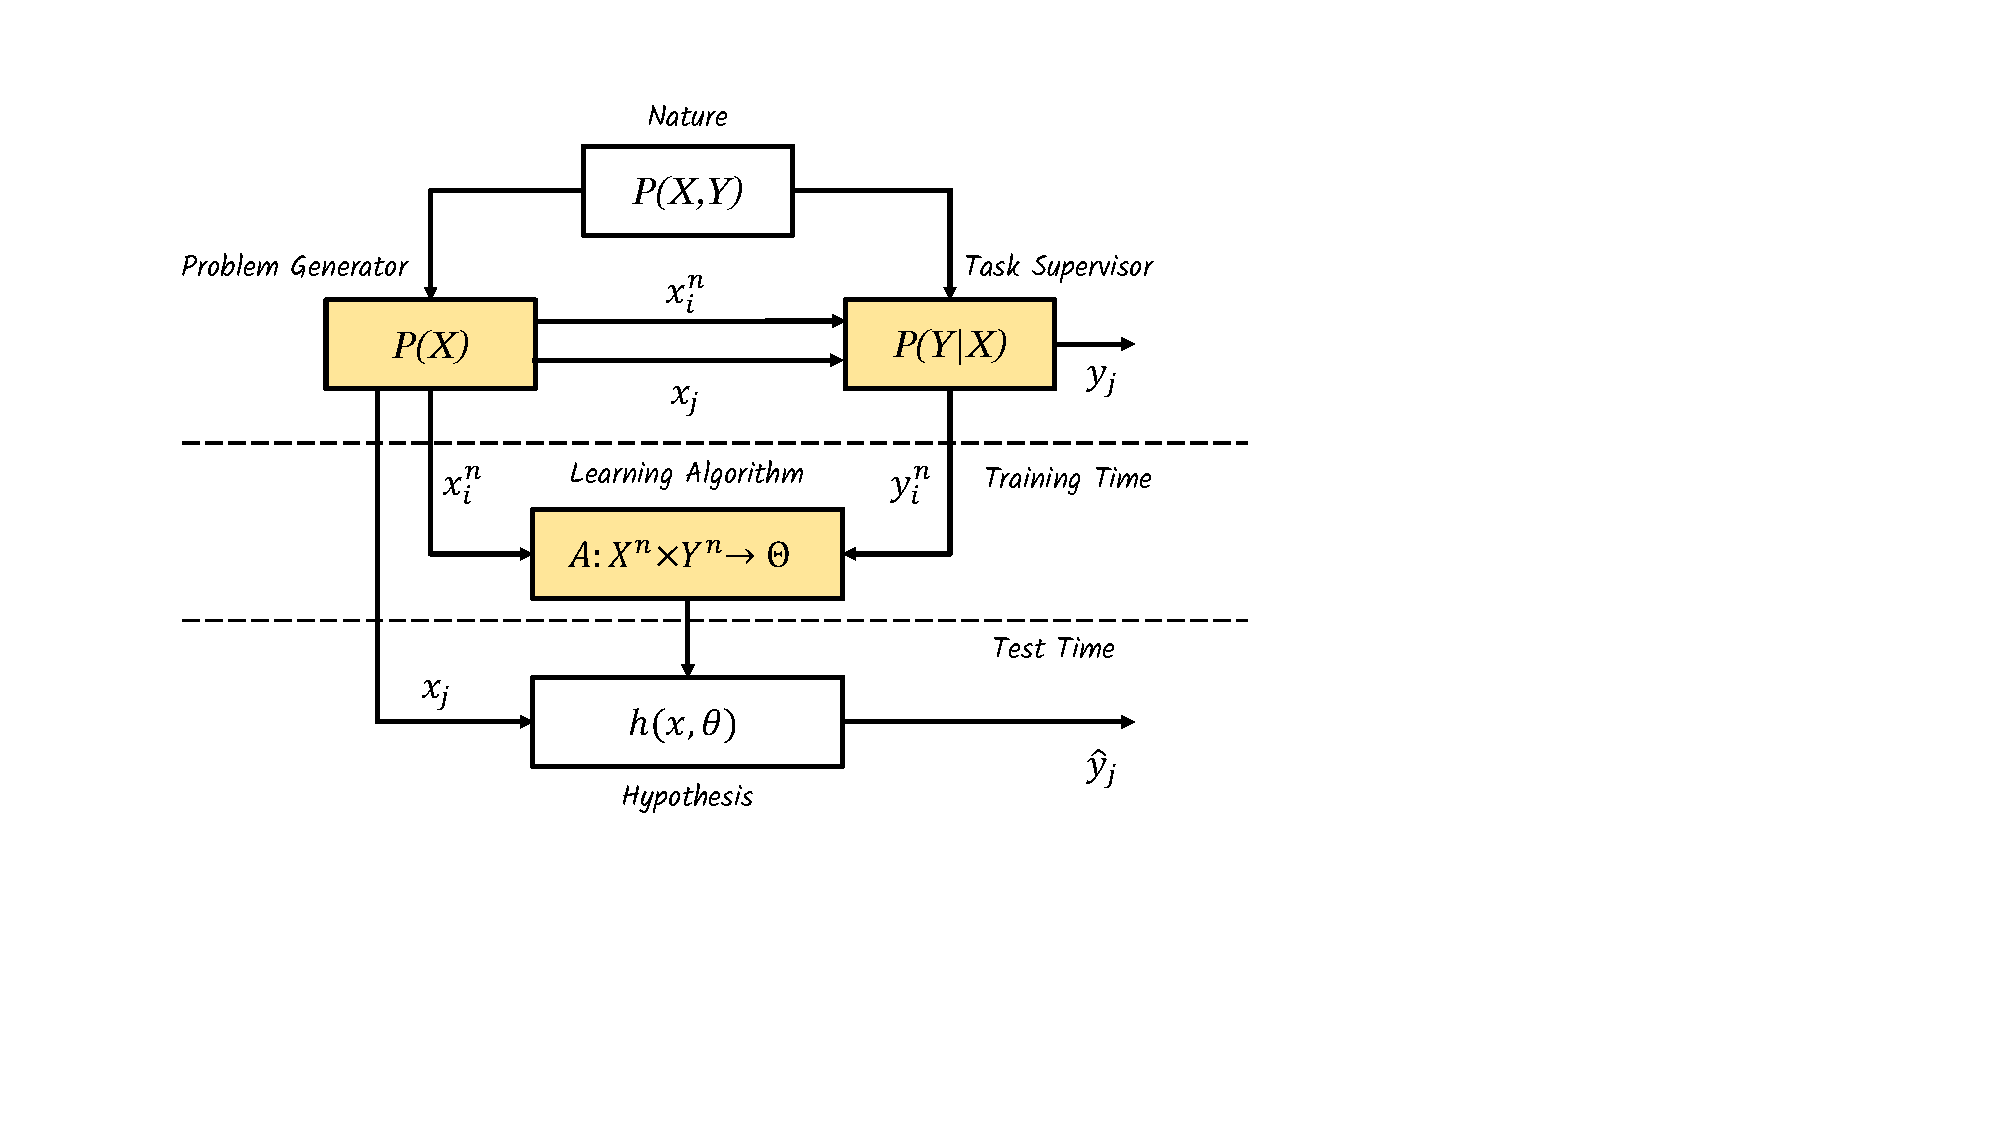
\includegraphics[width=
	\textwidth]{learning_settings_1}
	\caption{Problem setting.}\label{fig:problem_setting}
\end{figure}
\begin{enumerate}
	\item A \textbf{generator} of vectors randomly draw from a probability distribution \(P(\rvX)\), \(x\sim P(\rvX), x \in \XX \)\footnote{In \cref{ch:information}, we used $\sA_{\rvX}$ to represent the domain of $\rvX$ to emphasise that the domain was finite, it was an alphabet. Here we use $\XX$ to remember that this domain possibly is infinite.}, which represent instances of the problem\footnote{\(P(\rvX=\rx_i) = P_{\rvX}(\rx_i) = \sum_j P_{\rvX\rvY}(\rx_i, \ry_j) \therefore P_{\XX}\)is just a consequence of \(\PXY \therefore \rx \sim P_{\XX} \equiv \rx \sim P_{\rvX\rvY}\).};
	\item A \textbf{task supervisor} that knows the concept and returns an output vector \(\ry_i\) for every input vector \(\rx_i\):
	\begin{align}
		\ry_i = c(\rx_i) = P(\rvY \mid \rvX=\rx_i).
	\end{align}
	\item A \textbf{learning algorithm} \(\AA\) which is the functional that given a sample of \(n\) inputs and \(n\) outputs of a task, \(S_n = \{(\rx_1,\ry_1), \cdots, (\rx_n, \ry_n)\}\), selects a hypothesis \(h\) from the hypothesis space \(\HH\):
	\begin{align}
		\AA: \underbrace{(\XX \times \YY)^n}_{S_n} \to \HH .
	\end{align}
\end{enumerate}

The problem of learning is choosing from the \emph{hypothesis space}\footnote{Hypothesis spaces will be explained in \cref{hypothesis_space}.}, the one \emph{hypothesis} that best approximates the \emph{concept}. The selection is based on a training set of \(n\) i.i.d. observations drawn according to the unknown distribution \(\DD= \PXY\).

\subsection{Assumptions}\label{mlt_assumptions} The common assumptions are as follows~\cite{mello:2018, luxburg:2011}:
\begin{enumerate}
	[i.]
	\item \textbf{No assumption on \(\DD=\PXY\): } it can be any arbitrary joint probability distribution on \(\XX \times \YY\).\label{distribution-free}
	\item \textbf{\(\DD=\PXY\) is unknown at the training stage:} if not, learning would be trivial.
	\item \textbf{\(\DD=\PXY\) is fixed:} There is no ``time'' parameter, meaning that the ordering of examples in the sample is irrelevant\label{no-time}.
	\item \textbf{Independent sampling:} examples must be sampled in an identically independent manner (i.i.d.).\label{independent_sampling}
	\item \textbf{Labels may assume non-deterministic values:} due to noise or label overlap.
\end{enumerate}

\subsection{Hypothesis spaces}\label{hypothesis_space}
\begin{figure}
	[ht!] \centering
	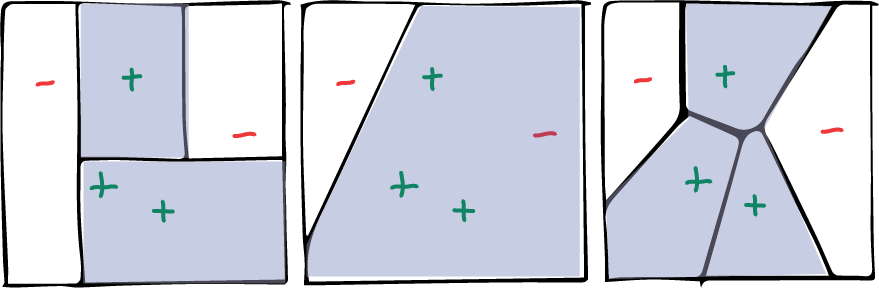
\includegraphics[width=0.7
	\textwidth]{hspaces}
	\caption{Different hypothesis spaces for the same sample.}\label{fig:hypothesis_spaces}
\end{figure}
The problem setting relies on the idea of a \emph{hypothesis space} (also known as a \emph{hypothesis class}). A hypothesis space is the set of all hypothesis generatable by a functional learning algorithm \( \AA\)\footnote{We can also say that the hypothesis space is the language defined by the learner.}. In the same hypothesis space \(\HH\), hypotheses are differentiated by their parameter vector \(\theta\). Choosing a hypothesis \(h_i\) is choosing its parameter \(\theta_i\).
\begin{align}
	h: \XX \times \Theta \to \YY, \\
	h(\rx) = p(\ry \mid \rx \land \theta),~ \theta \in \Theta.
\end{align}
Different learners will constraint the input space \(\XX\) differently (see \cref{fig:hypothesis_spaces}). Some algorithms are more complex than others, meaning they can express more different functions\footnote{We also use the term \emph{capacity} to describe this characteristic of learning algorithms to generate more complex hypotheses.}.

We usually call \(\HH_{all}\) the hypothesis space of all possible functions. However, generalisation only happens if a learner chooses a subset of \(\HH_{all}\) where to search for the hypothesis. The need for this constraint in generalisation, a bias, was prooved by~\citeauthor{mitchell:1980}: ``\emph{biases are [\dots] critical to the ability to classify instances that are not identical to the training instances}''. An intuitive argument for this is straightforward; if any function were allowed, the learner would be able to choose the function that ``memorises'' the sample, and that would certainly not generalise to other cases.

\subsection{Learning as error minimisation} Choosing from the \emph{hypothesis space}, the one \emph{hypothesis} \(h\) that \textbf{best} approximates the \emph{concept}, which we will call \(h_{\text{Bayes}}\), can be seen as an optimisation problem where we want to minimise the error of the approximation:
\paragraph{Absolute error} Let loss \(\ell:\YY \times \YY \to \Real \) be a measure of the error between the perfect output \(\ry\) of the supervisor, and the obtained output \(\hat{\ry}\) of the hypothesis. \textbf{The risk is the expected loss.} Find \(\theta_*\) which minimises the risk.
\begin{align}
	R_{\DD}(\theta) &= \E(\ell(\rx, \ry, h(\rx, \theta)), (\rx, \ry)\sim \DD, \theta \in \Theta\\
	\theta_{*}&= \argmin_{\theta \in \Theta} R(\theta)\\
	h(\rx,\theta_*) = h_{\text{Bayes}} &= \argmin_{h \in \HH} R(h)
\end{align}
The risk \(R_{\DD}\) is also called the absolute (or out-of-sample or theoretical) error of the hypothesis\footnote{\(R\), \(R(\theta)\) and \(R(h)\) are used interchangeably in this document.}. Nevertheless, there is one crucial caveat: \textbf{the choice of the loss metric is arbitrary, which curbs any objective, metric independent, interpretation of the results.}
\paragraph{Empirical error} The underlying difficulty of risk minimisation is that we are trying to minimise a quantity we cannot evaluate: if \(\PXY\) is unknown, we cannot directly compute the risk \(R(h)\) (absolute error). However, we can compute the risk of the hypothesis on the training sample:
\begin{align}
	\hat{R}_{S}(h) = \frac{1}{n} \sum_{i=1}^{n}(\ell(\rx_i, \ry_i, h(\rx_i)), (\rx,\ry)\sim S
\end{align}

With this empirical risk \(\hat{R}_{S}\) that we can evaluate, we find the hypothesis that minimises it. That is, given a sample \(S = \{(\rx_1,\ry_1),\cdots,(\rx_n, \ry_n)\}\), a hypothesis space \(\HH\), and a loss function \(\ell\), we define \(h_{\HH}\) as the function:
\begin{align}
	h_{\HH} = \argmin_{h\in \HH} \hat{R}_{S}(h)
\end{align}
According to the law of large numbers (\cref{law_of_large_numbers}), if the sample is large enough, by induction, a hypothesis generated optimising \(\hat{R}_{S}\) is close to \(R\). However, it is essential to notice that we still have to discuss at which rate does \(\hat{R}_{S}\) converge to \(R\) w.r.t. the sample size.


\section{Bias-Variance trade-off}\label{sec:bias-variance}
When we define a subset of \(\HH \subset \HH_{all}\) where to look for our hypothesis, we are imposing a constraint to the choice, a \emph{bias}. Besides, the subset \(\HH\) can be larger or smaller; for example, the hypothesis space of Neural Networks is much larger than the one of Perceptrons and also covers it \(\HH_{NN} \supset \HH_{\text{Perceptron}}\).
\begin{figure}
	[ht] \centering
	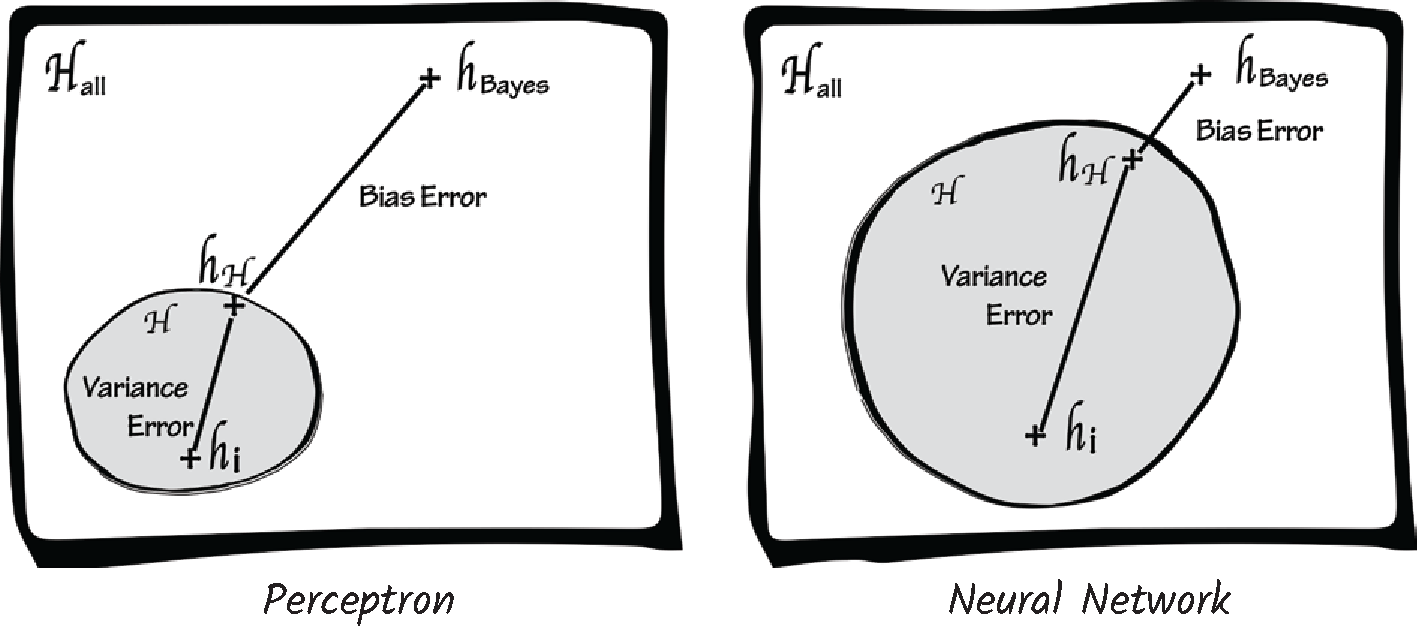
\includegraphics[width=1
	\textwidth]{bias_variance}
	\caption{Bias and variance errors}\label{fig:bias-variance} \end{figure}
Accordingly, we can distinguish two kinds of errors due to this constraint:
\begin{itemize}
	\item \textbf{Variance error:} represents how far a classifier \(h_i\) is from the best classifier in \(\HH\), \(h_\HH\). With a strong bias (small hypothesis space), any hypothesis \(h_i\) is expected to be closer to \(h_\HH\), there is less variance in the hypothesis space (see Figure~\ref{fig:bias-variance} Perceptron). Finding the best hypothesis in a larger hypothesis space is more laborious and, therefore, takes more resources (time and examples) than in a smaller one (see Figure~\ref{fig:bias-variance} Neural Network).
	\item \textbf{Bias error:} represents how far the classifier \(h_\HH\) is from the best classifier \(h_{\text{Bayes}}\). With larger, more complex, higher-order, hypothesis spaces we expect \(h_\HH\) to be closer to \(h_{\text{Bayes}}\) (see Figure~\ref{fig:bias-variance} Neural Network).
\end{itemize}
These two errors compound the generalisation gap, \(\Delta(h_i)\):
\begin{align}
	\Delta(h_i) &= R(h_i)-R(h_{\text{Bayes}}) \\
	&= \underbrace{(R(h_i)-R(h_\HH))}_{\text{Variance Error}}+ \underbrace{(R(h_\HH)-R(h_{\text{Bayes}}) )}_{\text{Bias Error}}
\end{align}
Machine learning practicioners will recognise here what is called \emph{overfitting} and \emph{underfitting}:
\begin{figure}
	[ht!] \centering
	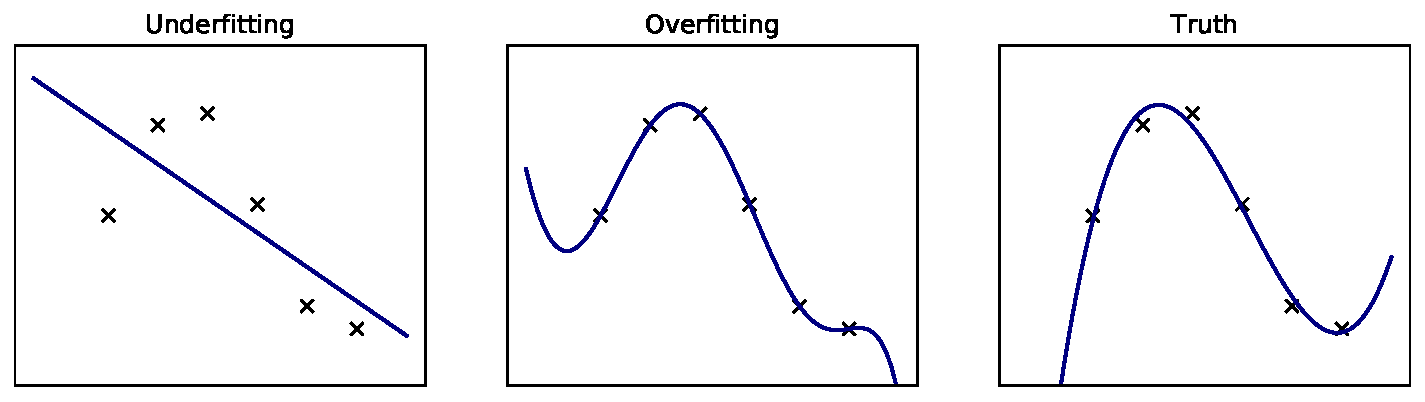
\includegraphics[width=0.9
	\textwidth]{curves}
	\caption{Example of underfitting and overfitting in a regression problem.}\label{fig:underfitting-overfitting} \end{figure}
\begin{itemize}
	\item \textbf{Overfitting:} bias error is small, but variance error is large; High variance is a consequence of fitting to random noise in the training data, rather than the intended outputs.
	\item \textbf{Underfitting:} bias error is large, but variance error is small; The bias error comes from wrong assumptions in the learning algorithm. Strong bias can cause an algorithm to miss relevant relations between inputs and outputs.
\end{itemize}
It is easy to notice that these two errors are conflicting: the stronger the bias, smaller is the \(\HH \subset \HH_{all}\), smaller is the variance error, but bigger is the bias error; and vice-versa (\cref{fig:generalisation_gap}). This trade-off is the central paradigm of Machine Learning Theory~\cite{slonim:2002}, its crucial challenge, and has different names underfitting-overfitting, precision-complexity, and performance-prediction.
\begin{figure}
	[ht!] \centering
	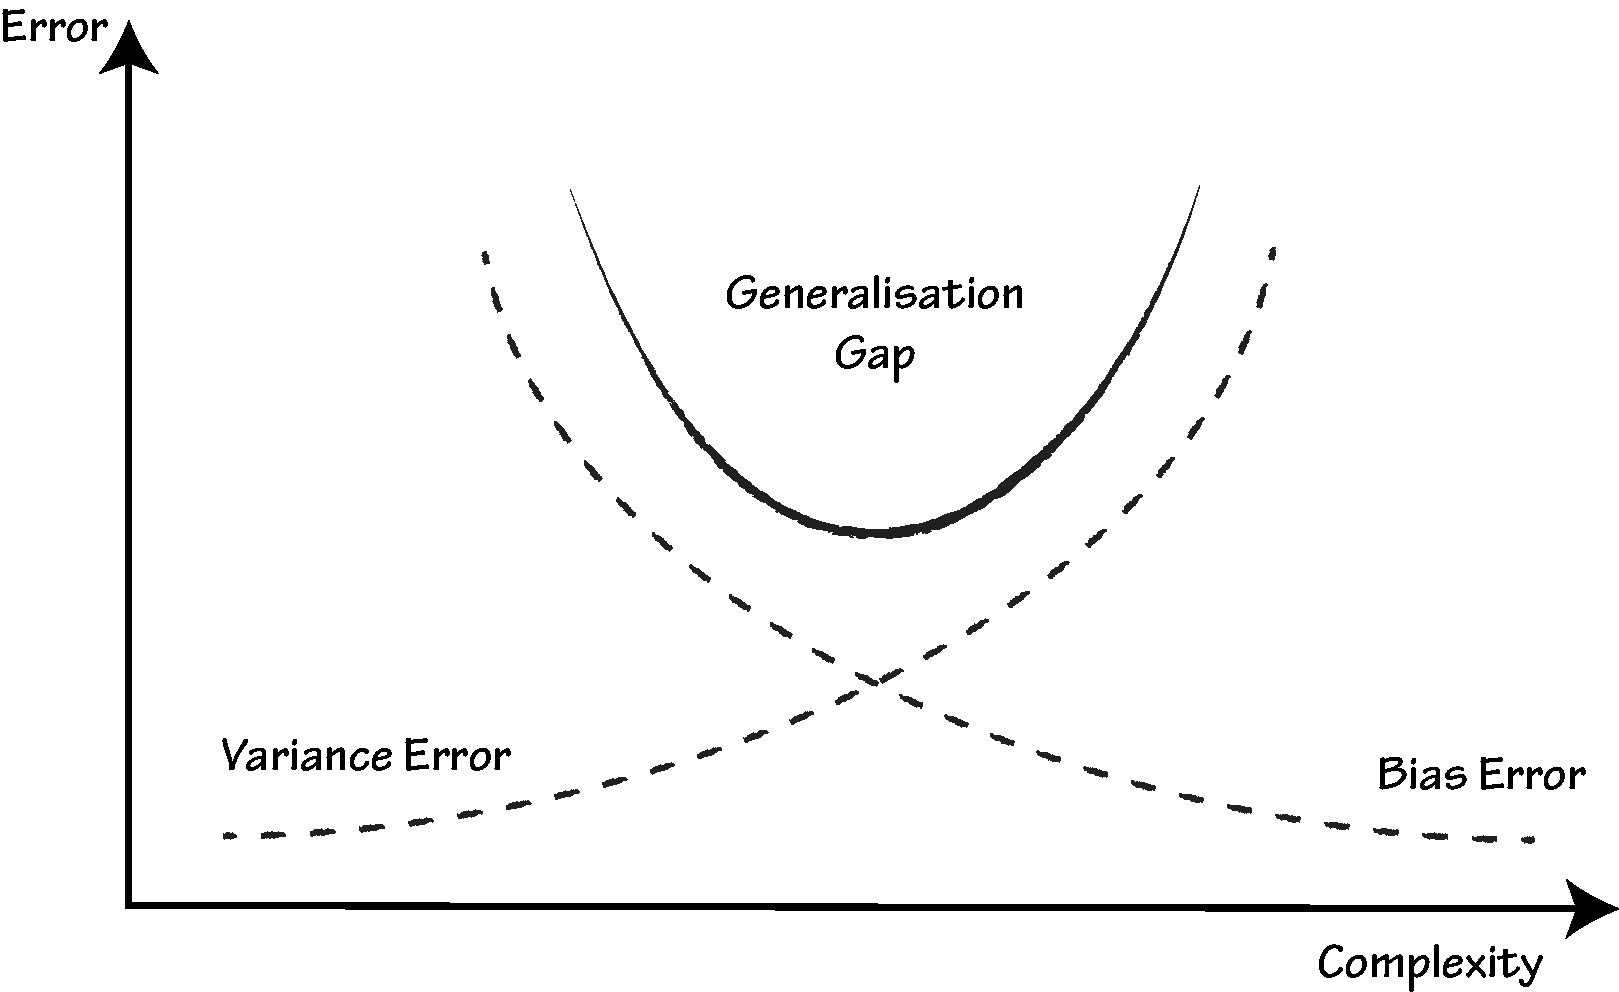
\includegraphics[width=0.8
	\textwidth]{generalisation_gap}
	\caption{Generalisation gap.}\label{fig:generalisation_gap}
\end{figure}
\textbf{The goal of machine learning algorithms is to come up with the simplest model that explains the data, but not simpler}.
\begin{quotation}
	\small \textit{ \flushright There are many more complicated explanations possible than simple ones. Therefore, if a simple explanation happens to fit your data, it is much less likely this is happening just by chance.\\
	\flushright ---~\citeauthor{blum:2007}\\
	}
\end{quotation}
\section{The PAC learning model}
Up to this point in the chapter, we have described MLT in accordance to \ac{SLT}. Now we will revisit some of what we already explained with the formalism of the PAC model.
\sidefigure{valiant}{0}{Leslie Valiant recieved the Turing Award in 2010.}
The PAC model was proposed by Leslie Valiant (see \cref{fig:valiant}) in 1984~\cite{valiant:1984}. The lack of citation to previous work from Vapnik and Chervonenkis is an indication that the overlap of CoLT and STL was reinvented. As expected, CoLT looks at the learning problem from a computational perspective, while SLT from a statistical one.

``The PAC framework deals with the question of learnability for a concept class \(\CC\) and not a particular concept''~\cite{mohri:2012}. The PAC model classifies concept classes in terms of their complexities to achieve an approximate solution; sample complexity, the number of examples needed, computation complexity, the number of iterations needed.

In the PAC framework, a \emph{concept} \(c\) is learnable if there is an algorithm capable of generating, with polynomial time and examples, a general function (the hypothesis \(h\)) that with high confidence (\(1-\delta\)), has an arbitrarily small error \(\epsilon\) in any given instance of the problem.
\begin{align}
	\underbrace{\text{ Probably }}_{\textrm{confidence} \geq(1-\delta)} \underbrace{\text{ Approximately }}_{\textrm{tolerance} \leq\epsilon} \underbrace{\text{ Correct }}_{h(\cdot)=c(\cdot)}
\end{align}

If, with absolute certainty, the hypothesis ``imitates'' the concept, \ie there is no error, we can say that there was learning:
\sidefigure{conceptVshypothesis}{0}{The concept versus the hypothesis.}

\begin{align}
	\exists h \in \HH: ~ P_{\rx \sim \DD}[c(\rx)\neq h(\rx)]=0 \to \text{learning}.
\end{align}
Nevertheless, this definition is too restrictive. For instance, if \(c \not \subset \HH\), there is no way of any \(h\) perfectly imitating \(c\). Let us redefine learning with these new relaxed constraints to the absolute error:
\begin{align}
	&P_{x \sim \DD}[c(\rx) \neq h(\rx)]= R_{\DD}(h)\\
	&\exists h \in \HH:~ R_{\DD}(h) \leq \epsilon, ~ 0 < \epsilon < \tfrac{1}{2} \to \text{learning}.
\end{align}
Allowing some tolerance to error, however, is still not sufficient. At one side, a \emph{hypothesis} does not need to be equal to the \emph{concept} to be \textbf{\emph{consistent} to the sample}, \ie to correctly predict every example of the sample. In the figure \ref{fig:conceptVShypothesis}, the hypothesis was \emph{lucky}, and there is no difference between the hypothesis and the concept for the particular sample, even though they are different maps of \(\XX\).

On the other side, it is possible that the sampling:
\begin{align}
	S_n = \{(\rx_1,\ry_1), \cdots, (\rx_n, \ry_n)\} \sim \DD^n
\end{align}
is \emph{unlucky}, and give the same kind of examples for the learning algorithm, an uninformative sample, making it impossible for the hypothesis to \emph{imitate} the concept for all \(\rx \in \XX\). In this \emph{unlucky} case, learning would be impossible. Hence, we relax the constraints once more:
\begin{align}
	\exists h \in \HH, ~0 < \epsilon < \tfrac{1}{2}, ~0 < \delta < \tfrac{1}{2}: \nonumber\\
	~P_{S \sim \DD^n}[R_{\DD}(h) > \epsilon] < \delta \to \text{learning}.
\end{align}
Nevertheless, if achieving such thresholds demands an unreasonable ammount of data and time, can we really say that learning has happened? What is a reasonable amount of time and examples?

Let \(d\) be a number such that representing any vector \(\rx \in \XX\) costs at most \(\OO(d)\) (\eg \(\XX = \Real^d\)), and \(\operatorname{size}(c)\) the computational cost of representing a concept \(c \in \CC\).
\begin{definition}
	A concept class \(\CC\) is \textbf{PAC-learnable} if there is a learning algorithm \(\AA\) and a polynomial function \(\operatorname{poly}(\cdot,\cdot, \cdot, \cdot, )\) such that for any \(0< \epsilon < \tfrac{1}{2}\) and any \(0< \delta < \tfrac{1}{2}\), for any distribution \(\DD\) on \(\XX\) and for any target concept \(c \in \CC\), the following holds for any sample size \(n \geq \operatorname{poly}(\tfrac{1}{\epsilon}, \tfrac{1}{\delta}, d, \text{size}(c))\)~\cite{mohri:2012}:
	\begin{align}
		P_{S \sim \DD^n}[R_{\DD}(h) \leq \epsilon] \geq (1 - \delta).
	\end{align}
	If \(\AA\) further runs in \(\operatorname{poly}(\tfrac{1}{\epsilon}, \tfrac{1}{\delta}, d, \text{size}(c))\), then \(\CC\) is said to be \textbf{efficiently PAC-learnable}. When such an algorithm \(\AA\) exists, it is called a \textbf{PAC-learning algorithm} for \(\CC\)~\cite{mohri:2012}.
\end{definition}


\section{PAC Bounds}
As we stated before, one of the main goals of \ac{MLT} is to guarantee bounds to the error and the number of samples needed (sample complexity) in learning problems. Here we present some of these guarantees as examples of how this theoretical development allows us to make claims on unknown distributions and unseen examples.
\subsection{Guarantees for finite hypothesis spaces --- consistent case}
\begin{theorem}[\cite{haussler:1988}]\label{th:haussler} Let \(\HH\) be a finite hypothesis space, \(\AA\) a learning algorithm that returns a consistent hypothesis \(h\), i.e.\ \(\hat{R}_{S}(h)=0\), for any hypothesis \(h\) and unknown distribution \(\DD=\PXY\).\\
	Let \(|S|=n\), then, \(\forall n \geq 1\):
	\begin{align}
		P[\exists h \in \HH: R_{\DD}(h)>\epsilon]\leq |\HH| e^{-\epsilon n}
	\end{align}
\end{theorem}
\begin{proof}
	Let \(h_{\text{bad}} (\text{bad} = 1, ..., k)\) be all hypotheses in the space \(\HH_{\text{bad}} \subset \HH\) where \( \forall h_{\text{bad}} \in \HH_{\text{bad}}: R_{\DD}(h_{\text{bad}})>\epsilon\), then:

	The chance of a \emph{bad} hypothesis to correctly predict an example is:
	\begin{align}
		P_{\rx_j\sim S}[(c(\rx_j) \neq h_{\text{bad}}(\rx_j))=\emptyset] \leq (1-\epsilon) \\
		P_{\rx_j\sim S}[R_{\rx_j}(h_{\text{bad}})=0] \leq (1-\epsilon)
	\label{haussler:a} \end{align}

	Therefore, the probability that a \emph{bad} hypothesis will predict all examples correctly in the training sample \(S_n\) is:
	\begin{align}
		P_{\rx_1 \sim S}[R_{\rx_1}(h_{\text{bad}})=0] &\land\\
		P_{\rx_2 \sim S}[R_{\rx_2}(h_{\text{bad}})=0] &\land\\
		\nonumber \cdots\\
		P_{\rx_n \sim S}[R_{\rx_n}(h_{\text{bad}})=0] &\leq \underbrace{(1-\epsilon) \cdots (1-\epsilon)}_{n} \\
		P[(\hat{R}_{S}(h)=0) \land (R_{\DD}(h)> \epsilon)] &\leq (1-\epsilon)^n
	\label{haussler:b} \end{align}
	We said there are \(k\) \emph{bad} hypotheses, then, the probability of any of these \emph{bad} hypothesis predicting correcly all the training sample is:
	\begin{align}
		P[h_1 \in \HH_{\text{bad}}: (\hat{R}_{S}(h_1)=0) \land (R_{\DD}(h)> \epsilon)] &\lor \\
		P[h_2 \in \HH_{\text{bad}}: (\hat{R}_{S}(h_2)=0) \land (R_{\DD}(h)> \epsilon)] &\lor \\
		\ldots \nonumber \\
		\lor P[h_k \in \HH_{\text{bad}}: (\hat{R}_{S}(h_k)=0) \land (R_{\DD}(h)> \epsilon)] &
		\leq \sum_{1}^k (1-\epsilon)^n\\
		P[\exists h \in H: (\hat{R}_{S}(h)=0) \land (R_{\DD}(h)>\epsilon)] &\leq k (1-\epsilon)^n
	\label{haussler:c} \end{align}
	Finally, as these \emph{bad} hypotheses belong to \(\HH_{\text{bad}} \subset \HH\), \(k < |\HH|\), therefore, we get the theoretical error of \(h\) given a precision tolerance of \(\epsilon\), and a sample complexity of \(n\) examples:
	\begin{align}
		P[\exists h \in \HH: R_{\DD}(h)>\epsilon]&\leq |\HH| (1-\epsilon)^n\label{haussler:d}\\
		(1-x) \leq e^{-x},&~0 \leq x \leq 1 \implies \nonumber\\
		P[\exists h \in \HH: R_{\DD}(h)>\epsilon]&\leq |\HH|e^{-\epsilon n}\label{haussler:e} \qedhere
	\end{align}
\end{proof}
From the PAC framework:
\begin{align}
	P[\exists h \in \HH: R_{\DD}(h)>\epsilon] < \delta
\end{align}
Therefore, Haussler theorem gives us a lower bound on the confidence:
\begin{align}
	\delta > |\HH|e^{-\epsilon n} \geq P[\exists h \in \HH: R_{\DD}(h)>\epsilon]\label{eq:delta}
\end{align}

We can rewrite the Haussler theorem to bound the number of examples needed for learning:
\begin{theorem}\label{th:sample_complexity}A learning algorithm \(\AA\) can learn a concept \(c\) from a class of concepts \(\CC\) with \(n < \frac{1}{\epsilon}(\ln{|\HH|}+\ln{\frac{1}{\delta}})\) training examples.
\end{theorem}
\begin{proof}
	\begin{align}
		\delta > |H|e^{-\epsilon n} \tag{from \eqref{eq:delta}}\\
		e^{-\epsilon n} < \frac{\delta}{|\HH|}\\
		- \epsilon n < (\ln{\delta} - \ln{|\HH|}) \\
		\epsilon n < (\ln{|\HH|} - \ln{\delta}) \\
		n < \frac{1}{\epsilon}(\ln{|\HH|} + \ln{\frac{1}{\delta}}) \\
		n \in \OO \biggl( \frac{1}{\epsilon}(\ln{|\HH|} + \ln{\frac{1}{\delta}})\biggr) \tag{sample complexity}\label{sample_complexity} \\
		\qedhere
	\end{align}
\end{proof}
Strangely, the sample complexity upper bound does not depend on \(\CC\) or \(\DD\) but depends logarithmically to the size of \(\HH\)~\cite{haussler:1988}.

\subsection{No free lunch theorem}
\paragraph{Is a universal concept class learnable?} Let \(\XX=\{0,1\}^{d}\), the space of Boolean vectors of size \(d\). A universal concept class \(\UU_d\) has all subsets of \(\XX\), i.e. contains all possible classifications for a given instance space \(\XX\).
\begin{align}
	|\UU_d| = 2^{|\XX|}&=2^{(2^d)} \\
	|\HH| &\geq |\UU_d| \\
	|\HH| &\geq 2^{(2^d)}
\end{align}
From Theorem \ref{th:sample_complexity}:
\begin{align}
	n &\in \OO \biggl( \frac{1}{\epsilon}(\ln{|\HH|} + \ln{\frac{1}{\delta}})\biggr)\\
	n &\in \OO \biggl( \frac{1}{\epsilon}(2^d \ln(2) + \ln{\frac{1}{\delta}})\biggr) \therefore\\
	n &\in \OO \biggl( 2^d; \frac{1}{\epsilon}; \ln{\frac{1}{\delta}} \biggr)
\end{align}
Therefore, the sample complexity is not polynomial to \(d\), and \textbf{\(\UU_d\) is not PAC Learnable}. The ``no free lunch'' theorem~\cite{wolpert:1997} states there is no universal concept, therefore, no universal learning algorithm for all tasks. Specifically, averaged over all possible data generating distributions, every classification algorithm achieves the same error when classifying previously unknown points.

\subsection{Guarantees for finite hypothesis spaces --- inconsistent case} Usually, there is no hypothesis in \(\HH\) consistent with the training sample due to the stochastic nature of the supervisor or the concept class being more complex than the hypothesis class used by the learning algorithm.

To derive bounds for this inconsistent case, we will use the ``law of large numbers''.

\paragraph{Law of large numbers}\label{law_of_large_numbers} The law of large numbers states that the mean of random variables \(\xi_i\), drawn i.i.d. from some probability distribution \(P\), converges to the mean of \(P\) itself when the sample size goes to infinity.
\begin{align}
	&\text{for}~n \to \infty, \nonumber\\
	&\frac{1}{n} \sum_{i=1}^{n}\xi_i \to \mathbb{E}(\xi), \xi_i \sim P.
\end{align}

Based on the fact that a statistic\footnote{Remember: A statistic is a function of random variables that does not depend on parameters.} of random variables can be treated as a random variable, we can make the loss function \(\ell(\rx, \ry, h(\rx))\) be the random variable \(\xi\) from above. From what we can conclude that for a fixed \(h\), the empirical risk converges to the theoretical risk as the sample size goes to infinity:
\begin{align}
	&\text{for}~n \to \infty, \nonumber\\
	&\hat{R}_{S}(h) = \frac{1}{n} \sum_{i=1}^{n}(\ell(\rx_i, \ry_i, h(\rx_i)) \to \mathbb{E}(\ell(x, y, h(\rx))=R(h).
\end{align}

\paragraph{Chernoff-Hoeffding inequality} Moreover, we can use the famous \emph{Chernoff-Hoeffding's inequality} to bound the approximation of the risk:
\begin{align}
	P \left(\Bigg | \frac{1}{n} \sum_{i=1}^{n}\xi_i - \mathbb{E}(\xi) \Bigg | \geq \epsilon \right) &\leq 2 e^{(-2n\epsilon^2)} \tag{Chernoff-Hoeffding's inequality}\\
	P(|\hat{R}_{S}(h) - R(h)| \geq \epsilon) &\leq 2 e^{(-2n\epsilon^2)}
\end{align}

Unfortunately, this bound only holds for a fixed-function \(h\) which does not depend on the training data, but our hypothesis certainly does depend. The reason for such constraint is intuitive. If we let the hypothesis space convey all possible functions and do not restrict our hypothesis to be independent of the training data, we can always generate a function that ``memorises'' the given sample and has no empirical error. Such function will most certainly not generalise well and invalidate the bound.

Vapnik and Chervonenkis solved this conundrum by using the union bound.

\paragraph{Union bound} Even if we are not allowed to select a hypothesis from the space using training data, the bound still holds for any hypothesis taken at random. Also, if we enumerate all the functions in \(\HH\), using the fact that it is finite, the bound still holds for each hypothesis:
\begin{align}
	P(|\hat{R}_{S}(h_1) - R(h_1) | > \epsilon) &\lor \nonumber \\
	P(|\hat{R}_{S}(h_2)-R(h_2)| > \epsilon) &\lor \cdots \nonumber \\
	P(|\hat{R}_{S}(h_{|\HH|})-R(h_{|\HH|})| > \epsilon) &\leq \sum^{|\HH|} 2 e^{(-2n\epsilon^2)} \\
	\therefore P(\sup_{h \in \HH}|\hat{R}_{S}(h) - R(h)| >\epsilon) &\leq 2 |\HH| e^{(-2n\epsilon^2)}\\
	P\left[ \exists h \in \HH:~|\hat{R}_{S}(h) - R(h)| >\epsilon\right] &\leq 2 |\HH| e^{(-2n\epsilon^2)}
\label{eq:union_bound} \end{align}
\begin{theorem}\label{thrm:finite-inconsistent}
	Let \(\HH\) be a finite hypothesis class. Then, for any \(0 < \delta < \tfrac{1}{2}\), with probability at least \(1-\delta\), the following innequality holds~\cite{mohri:2012}:
	\begin{align}
		\forall h \in \HH,~&R(h)\leq \hat{R}_{S}(h) + \epsilon \nonumber \\
		&R(h)\leq \hat{R}_{S}(h) + \sqrt{\frac{\ln{|\HH|}+ \ln{2/\delta}}{2n}}
	\end{align}
\end{theorem}
\begin{proof}
	\begin{align}
		P\left[ \exists h \in \HH:~|\hat{R}_{S}(h) - R(h)| >\epsilon\right] &< \delta \tag{from PAC}\\
		P\left[ \exists h \in \HH:~|\hat{R}_{S}(h) - R(h)| >\epsilon\right] &\leq 2 |\HH| e^{(-2n\epsilon^2)} \tag{from \eqref{eq:union_bound}}\\
		\therefore \delta &> 2 |\HH| e^{(-2n\epsilon^2)}
	\end{align}
	Assuming \(\delta = 2 |\HH| e^{(-2n\epsilon^2)}\), we have:
	\begin{align}
		e^{(-2n\epsilon^2)} = \frac{\delta}{2|\HH|} \\
		-2n\epsilon^2 = \ln{\delta} - ln{2|\HH|}\\
		\epsilon^2 = \frac{\ln{|\HH|}+\ln{2}-\ln{\delta}}{2n}\\
		\therefore \epsilon > 0 \rightarrow \epsilon = + \sqrt{\frac{\ln{|\HH|}+ \ln{2/\delta}}{2n}}\label{eq:epsilon_ch}
	\end{align}
	By definition, \(R(h)\geq \hat{R}_{S}(h)\), thus:
	\begin{align}
		P\left[ \exists h \in \HH:~(R(h) - \hat{R}_{S}(h)) >\epsilon\right] &< \delta \\
		P\left[ \forall h \in \HH:~(R(h) - \hat{R}_{S}(h)) \leq \epsilon\right] &\geq 1 - \delta
	\end{align}
	Therefore, with probability at least \(1-\delta\):
	\begin{align}
		\forall h \in \HH, R(h)&\leq \hat{R}_{S}(h) + \epsilon \\
		\forall h \in \HH, R(h)&\leq \hat{R}_{S}(h) + \sqrt{\frac{\ln{|\HH|}+ \ln{2/\delta}}{2n}}\label{eq:finite_inconsistent_epsilon}\tag{from \eqref{eq:epsilon_ch}}\\
		\forall h \in \HH, R(h)&\leq \hat{R}_{S}(h) + \OO \left(\sqrt{ \log |\HH| }; \sqrt{1/n}; \sqrt{ \log 1/\delta} \right)
	\end{align}
\end{proof}
We can rewrite theorem \ref{thrm:finite-inconsistent} to bound the sample complexity:
\begin{theorem}
	A learning algorithm \(\AA\) can learn a concept \(c\) from a class of concepts \(\CC\) with \(n \leq \frac{\ln{|\HH|}+\ln{\frac{2}{\delta}}}{2\epsilon^2}\) training examples.
\end{theorem}
\begin{proof} \ref{eq:finite_inconsistent_epsilon},
	\begin{align}
		\epsilon \leq \sqrt{\frac{\ln{|\HH|}+ \ln{2/\delta}}{2n}}
		\therefore n \leq \frac{\ln{|\HH|}+ \ln{2/\delta}}{2\epsilon^2}
	\end{align}
\end{proof}

\subsection{Guarantees for infinite hypothesis space --- inconsistent case} It can be argued that for our use in machine learning, there is no need for guarantees for infinite \(\HH\) due to the nature of computer hardware and their memory limitations, which already discretise the hypothesis spaces. Therefore, we will give a general idea of this case.

One of the most striking insights of Vapnik and Chervonenkis is the idea of the \emph{shattering coefficient} (\(\NN\)). Let us take a look at the bound for finite inconsistent case (Theorem \ref{thrm:finite-inconsistent}):
\begin{align}
	&\forall h \in \HH,\nonumber\\
	&R(h)\leq \hat{R}_{S}(h) + \sqrt{\frac{\ln{|\HH|}+ \ln{2/\delta}}{2n}} \tag{finite hypothesis space, inconsistent case}
\end{align}
The \(\ln |\HH|\) relates to \(d\), the size of the \emph{representation} of the hypothesis space. Another remark worth mentioning is that in the union bound we just added the probabilities of each \(h_i \in \HH\) without considering where \(P(h_j) \cap P(h_k), j \neq k\).
\begin{figure}
	[ht!] \centering
	\begin{venndiagram2sets}
		[tikzoptions={fill opacity=0.5},shade=blue!50!white, radius=0.8cm, labelA={\(h_j~~\)}, labelB={\(~~h_k\)}] \fillA \fillB
	\end{venndiagram2sets}
	\caption{\(P(h_j) \cap P(h_k)\) is summed twice in the union bound.}
\label{fig:join_probability} \end{figure}

In reality, there are several different \(h \in \HH\) that provide the same map \(x \in S \to y \in \YY\). Therefore, the effective size of \(\HH\) is smaller than \(|\HH|\). Using a symmetrisation trick~\cite[section 5.2] {luxburg:2011}, Vapnik and Chervonenkis showed that there is at most \(2^{2n}\) effectively different hypothesis. In the PAC framework, \(|\YY|=2\), so if a pattern is a set \(\{y_1,\cdots,y_n\}\), there are \(|\HH|=2^n\) different patterns, thus, effectively different hypothesis. This number, however, can be even smaller; for example, a certain \(y_k, k<n\) can, for example, only accept the value \({+}\). The shattering coefficient is a growth function, \ie it measures the number of effectively distinct hypotheses as the sample size \(n\) grows. It is a capacity measure of a hypothesis class. Whenever \(\NN(\HH, n)=2^n\), there exists a sample of size \(n\) on which all possible separations of the patterns can be achieved by some \(h \in \HH\).

We can now rewrite theorem \ref{thrm:finite-inconsistent} as:
\begin{align}
	\forall h \in \HH&,\nonumber\\
	R(h)&\leq \hat{R}_{S}(h) + \sqrt{\frac{\ln{\NN(\HH, n)}+ \ln{2/\delta}}{2n}}
\end{align}
Another capacity measure is the famous VC dimension\footnote{Named after Vapnik and Chervonenkis.}.
\begin{align}
	\operatorname{VC}(\HH)=max\{n \in \mathbb{N}| \NN(\HH, n)=2^n \text{ for some }S_n\}
\end{align}
A combinatorial result relates the growth behaviour of the shattering coefficient with the VC dimension:
\begin{theorem}
	[Vapnik, Chervonenkis, Sauer, Shelah]
	\begin{align}
		\text{If }&\operatorname{VC}(\AA)=d, \forall n \geq 1,\nonumber
		 ~&\NN(\HH, n) \leq \sum_{k=0}^d \binom{n}{k} \leq\left(\frac{\epsilon n}{d}\right)^d
	\end{align}
\end{theorem}

%
\section{Minimum Description Length}
\section{PAC-Bayes}
For a long time, \ac{MLT} was divided between Bayesian inference and PAC learning. In 1997, \citeauthor{shawe-taylor:1997} first presented a theorem of PAC guarantees for Bayesian algorithms (algorithms that minimise the risk using a prior probability for the data and hypothesis)\cite{shawe-taylor:1997}. This bridge allowed tighter PAC bounds for learning algorithms that take advantage of informative priors. Here we give PAC Bayes bounds for finite hypothesis spaces (for more, see \cite{mcallester:1999} and \cite{macallester:2013}).
\subsection{PAC Bayes Bound Guarantees for finite hypothesis spaces --- consistent case}

\begin{theorem}[Pre. Th. 1 \cite{mcallester:1999}] Let \(\HH\) be a finite hypothesis space, \(\AA\) a learning algorithm that returns a consistent hypothesis \(h\), i.e.\ \(\hat{R}_{S}(h)=0\), for any hypothesis $h$ and unknown distribution \(\DD=\PXY\), any \(|S|=n: n \geq 1\). For any probability distribution $P$ assigning nonzero probability to every hypothesis in a finite hypothesis space \(\HH\), with confidence $1-\delta$ over the selection of the sample of $n$ instances the following holds true:\\
	\begin{align}
		P[h \in H: (\hat{R}_{S}(h)=0) \land (R_{\DD}(h)>\epsilon)]\leq \frac{\ln \frac{1}{P(h)}+ \ln \frac{1}{\delta}}{n}
	\end{align}
\end{theorem}
\begin{proof}
	This proof is very similar to the one in Theorem \ref{th:haussler}. From \eqref{haussler:c}:
	\begin{align}
		P[h \in H: (\hat{R}_{S}(h)=0) \land (R_{\DD}(h)>\epsilon)] &\leq (1-\epsilon)^n,
	\end{align}
	But we also know that:
	\begin{align}
		P[h \in H: (\hat{R}_{S}(h)=0) \land (R_{\DD}(h)>\epsilon)] &\leq P(h)\delta\\
		(1-x) \leq e^{-x},~0 \leq x \leq 1 &\implies \nonumber\\
		e^{-\epsilon n} &< P(h) \delta\\
		\epsilon &< \frac{\ln \frac{1}{P(h)}+ \ln \frac{1}{\delta}}{n} \\
		\nonumber \qedhere
	\end{align}
\end{proof}
\subsection{Guarantees for finite hypothesis spaces --- inconsistent case}
\begin{theorem}[Pre. Th. 2 \cite{mcallester:1999}] Let \(\HH\) be a finite hypothesis space, \(\AA\) a learning algorithm that returns a consistent hypothesis \(h\), i.e.\ \(\hat{R}_{S}(h)=0\), for any hypothesis $h$, unknown distribution \(\DD=\PXY\),  sample \(|S|=n: n \geq 1\), and probability distribution $P$ assigning nonzero probability $\forall h \in \HH$, with confidence $(1-\delta)$the following holds true:\\
	\begin{align}
		\forall h \in \HH,~R(h)\leq\hat{R}_{S}(h) + \sqrt{\frac{\ln{\frac{1}{P(h)}}+ \ln{\frac{2}{\delta}}}{2n}}
	\end{align}
\end{theorem}
\begin{proof}
	As in Theorem \ref{thrm:finite-inconsistent}, we need to apply the union bound over the Chernoff bound:
	\begin{align}
		P[h \in H: (\hat{R}_{S}(h_1)=0) \land (R_{\DD}(h)>\epsilon)] &\leq 2e^{(-2n\epsilon^2)},
	\end{align}
	But we also know that:
	\begin{align}
		P[h \in H: (\hat{R}_{S}(h)=0) \land (R_{\DD}(h)>\epsilon)] &\leq P(h)\delta \\
		2e^{(-2n\epsilon^2)} &< P(h) \delta\\
		\epsilon &< \sqrt{\frac{\ln{\frac{1}{P(h)}}+ \ln{\frac{2}{\delta}}}{2n}}\\
		\nonumber \qedhere
	\end{align}
\end{proof}

\section{Critiques on MLT}
This dissertation aims to present an emergent new theory for understanding Deep Learning. In this context, we should first ask ourselves:  \textbf{What is wrong with current \ac{MLT}? Do we need a new theory?}

Truth be told: we did not cover \emph{current} \ac{MLT} in this chapter which aimed to be an introductory overview to the subject. There are many topics in active development beyond what was presented here: Structural Risk Minimisation, Rademacher complexity, Uniform Stability, for example.

With this caveat, here we digest some of the critiques on the current state of MLT in two parts, one for general critiques and another for critiques specific to the case of Deep Learning.

\subsection{General critiques}\label{sec:general_critiques}
\paragraph{No assumption on \(\DD=\PXY\) (see \ref{assumptions}, assumption \ref{distribution-free}): } One of the assumptions of classical learning theory is that ``there are no assumptions on \(\DD=\PXY\)''. Although this assumption means that MLT bounds guarantee approximation to any arbitrary distribution, the ones of practical interest are distributions found in Nature. These practical distributions have some peculiar characteristics that physicists know about~\cite{lin:2016}: Low polynomial order, locality, symmetry, among others.
\paragraph{Absence of the notion of ``time''(see \ref{assumptions}, assumption \ref{no-time}): } One of MLT assumptions on \(\PXY\) is that it is fixed, there is no ``time'' parameter. Several practical uses of machine learning are in data streams where it is common to have one observation affecting the probability of the future ones~\cite{mello:2018}.
\paragraph{Identically Independent sampling (see \ref{assumptions}, assumption \ref{independent_sampling}): } One of the assumptions of Machine Learning is that the datasets are sampled i.i.d. This sampling assumption is often violated in practice; for example, a machine learning medical application may use data from one hospital to train a model that will be applied worldwide.

The violations are, of course, of practical reasons. However, up to what point can we say that a particular dataset is i.i.d.? Let us think over the problem of facial recognition. Taking photos at random in a university is not i.i.d because the people that goes to the university is a biased set of the whole population. If we use random images on the Internet, we may only get the kind of picture people chose to display, a bias of intention. There is always some bias in any dataset: a selection, intention bias or technical bias.

\paragraph{Arbitraty Loss metrics} In \ac{MLT} learning setting, the choice of the loss function is arbitrary, which curbs any objective, metric-independent interpretation of the results.

% \paragraph{Conflicting optimisation objectives} Bias and variance are two conflicting objectives that the learning algorithm tries to minimise. It would be more practical if it were a single-sided optimisation problem\cite{slonim:2002}.

\subsection{In specific for Deep Learning}
\paragraph{Vacuous bounds}
Machine Learning Theory cannot explain deep neural networks generalisation performance. Deep learning generalisation gap, according to \ac{MLT}, is in \(\OO(|\theta| \log |\theta|)\), where \(|\theta|\) is the number of parameters of the network~\cite{kakade:2008}. These bounds are vacuous by orders of magnitudes~\cite{zhou:2019, zhang:2016}. However, deeper and larger networks consistently show better generalisation performance than smaller ones.
\paragraph{``Inexplicable'' phenomena} \acf{DL} has several phenomena with no definitive explanation, stemming from a single narrative.
\begin{itemize}
	\item Generalisation with more layers: as we explained in this chapter, the current \acs{MLT} expects models with fewer parameters to generalise better; that is not what happens in \acs{DL}. Moreover,~\citeauthor{zhang:2016} showed that the hypothesis space of \acs{DNN} is large enough to allow convergence to random labels.
	\item Disentanglement of semantic factors: the representation of the input in deep layers disentangle semantic factors, \ie different semantic factors are not strongly correlated in the representation;
	% \item Flat minimum and SGD: Flat minima are points in a function located in a ``valley'', \ie the gradient to the neighbourhood is small. \acs{SGD} algorithm running on \acp{DNN} seem to have a \emph{preference} for finding minima which are in such ``valleys'', thus, a preference for \emph{flat minima}. This property of \acs{DL} is crucial for generalisation. Still, there is no consensus on why this phenomenon occurs.
	\item Superconvergence:~\citeauthor{smith:2019} present that overall training time can be shortened and better accuracy achieved by the usage of cyclical learning rates.~\citeauthor{howard:2018universal} propose a slight variation of the method, slanted triangular learning rates, and achieve even better performance. This superconvergence phenomenon is not well studied, and there are only a few conjectures on why it does happen.
	\item Critical Learning Periods:~\citeauthor{achille:2018critical} show that ``similar to humans and animals, deep artificial neural networks exhibit critical periods during which a temporary stimulus deficit can impair the development of a skill.'' This finding questions the assumption that the order in which a model experience evidence does not affect learning.
\end{itemize}
\section{Concluding Remarks}
Most of the general critiques in \cref{sec:general_critiques} are not problems of current \ac{MLT} but choices\footnote{Teo: this is an observation from Moacir, should I cite? How?}.
Specific to Deep Learning, however, \citeauthor{zhang:2016} clearly challenges current \ac{MLT} concept of generalisation based on the expressivity of the model\cite{zhang:2016}.  They show that the expressivity of neural networks is sufficient to easily fit random labels and can memorize the entire dataset. As randomizing labels is a data transformation that do not affect the generalisation performance in current \ac{MLT} generalisation bounds. Moreover, they show that explicit regularisation may improve generalisation, but is neither necessary or sufficient. While implicit regularisation happens for models trained with SGD even without explicit regularizers.

Current \ac{MLT} sample complexity and generalisation bounds based on the size of the hypothesis space focus research attention to models architectures. These findings show that Deep Learning is more than \acp{DNN} and that at least the optmiser has a role in generalisation.

One of the most strong critiques to the theory concerning Deep Learning has always been the lack of non-vacuous bounds. Recently, however, \cite{dziugaite:2017} presented non-vacuous generalisation bounds. But it is important to notice that they did so by not only using PAC-Bayes bounds but also exploring the ``flatness''/location of minima found by SGD.

Without disregarding the immense contribution of \cite{dziugaite:2017} the paper does not pretend to solve the conceptual problems in \ac{MLT}. Understanding Deep Learning, indeed, requires rethinking generalisation. A new learning theory may bring a new narrative that unifies the explanations for Deep Learning phenomena. Despite its many weaknesses \acf*{IBT} presents a new narrative.


% Understanding deep networks requires rethinking generalisation
% . The experiments we conducted emphasise that the
% effective capacity of several successful neural network architectures is large enough to shatter the
% 2This conv-net is the Coates & Ng (2012) net, but with the filters selected at random instead of with k-means.
% training data. Consequently, these models are in principle rich enough to memorise the training data.
% This situation poses a conceptual challenge to statistical learning theory as traditional measures of
% model complexity struggle to explain the generalisation ability of large artificial neural networks.
% We argue that we have yet to discover a precise formal measure under which these enormous models
% are simple. Another insight resulting from our experiments is that optimisation continues to be
% empirically easy even if the resulting model does not generalise. This shows that the reasons for
% why optimisation is empirically easy must be different from the true cause of generalisation.
%

% Generalization in Deep Learning
% However, a recent paper (Zhang et al., 2017) has empirically shown that successful deep hypothesis spaces have sufficient capacity to memorize random labels. This observation has been called an “apparent paradox” and has led to active discussion by many researchers (Arpit et al., 2017; Krueger et al., 2017; Hoffer et al., 2017; Wu et al., 2017; Dziugaite and Roy, 2017; Dinh et al., 2017). Zhang et al. (2017) concluded with an open problem stating that understanding such observations require rethinking generalization, while Dinh et al. (2017) stated that explaining why deep learning models can generalize well, despite their overwhelming capacity, is an open area of research.

% \section{Conclusion} Performance-Complexity as central paradigm
